\documentclass[
	12pt,
	a4paper,
	DIVcalc,
	titlepage,
	twoside,
	liststotoc,
	bibtotocnumbered
]{scrbook}

%\usepackage[parfill]{parskip}    % Activate to begin paragraphs with an empty line rather than an indent
\usepackage[utf8]{inputenc}     %% dt. Umlaute mit utf-8, 
\usepackage[ngerman]{babel}
\usepackage{amsmath}
\usepackage{amsfonts}
\usepackage{amssymb}
\usepackage{graphicx}
\usepackage{algorithmic}
\algsetup{indent=1.7em}
\usepackage{natbib}
%\bibpunct{(}{)}{;}{a}{}{,} % to follow the A&A style

\usepackage[
	automark,		% Kapitelangaben in Kopfzeile automatisch erstellen
        headsepline,		% Trennlinie unter Kopfzeile
%        footsepline,
	ilines			% Trennlinie linksbündig ausrichten
]{scrpage2}
\pagestyle{scrheadings}

\usepackage[a4paper, bookmarks, colorlinks]{hyperref}	%%farbige Hyperlinks 
\hypersetup{%
	pdfkeywords = {},
	linkcolor = black,
	urlcolor = black,
	menucolor=black,
	citecolor = black,
	pagecolor=black,
	bookmarksopen = true, 
	bookmarksnumbered = true,
	pdfpagemode = {UseNone}, % UseNone, UseThumbs,UseOutlines, FullScreen
	pdfstartview = {} % ohne (nicht None), Fit, FitB
	%pdfcreator = {Adobe-Acrobat-Distiller},
	%pdfproducer = {LaTeX with hyperref and thumbpdf}
}

\begin{document}

\frontmatter
	\titlehead{Christian--Albrechts--Universit"at zu Kiel\\ Institut f"ur Theoretische Physik und Astrophysik}
	\subject{Diplomarbeit}
	\title{L"osung des Strahlungstransportproblems in Pfadintegralform mit effizienten Monte--Carlo--Verfahren}
	\author{vorgelegt von Thies Heidecke\\(theidecke@astrophysik.uni-kiel.de)}
	\publishers{betreut durch Prof. Sebastian Wolf}
	\date{Version vom \today}
	\maketitle
	% standard-titelblatt verf"ugbar?

	\tableofcontents	%%Inhaltsverzeichnis
	%\listoffigures	%%Abbildungsverzeichnis
	%\listoftables		%%Tabellenverzeichnis

	\newcommand{\location}[1]{\mathbf{#1}}
	\newcommand{\scatter}[1]{\overset{#1}{\leftrightsquigarrow}}
	\newcommand{\normalized}[1]{\frac{#1}{||#1||}}

\mainmatter
		\chapter{Einleitung}
	\section{Motivation}
	TODO: astrophysikalischer Kontext $\rightarrow$ Begr"undung der in Sektion (\ref{sec:radiative_transfer}) gemachten Annahmen
	\section{Ziele der Arbeit}
	In dieser Arbeit soll eine Pfadintegraldarstellung der Strahlungstransportgleichung hergeleitet werden, sowie dessen Nutzen f"ur Monte--Carlo--Verfahren zur L"osung des Strahlungstransportproblems theoretisch und praktisch in Form eines Computerprogrammes gezeigt werden.
	
	\section{Nomenklatur}\label{subsec:nomenklatur}
	Im folgenden Text werden die in Tabelle \ref{tab:nomenklatur} angegebenen Schreibweisen benutzt.

	\begin{table}
		\caption{Nomenklatur}
		\begin{center}
		\begin{tabular}{rll}
			Schreibweise & Bedeutung & Einheit \\
			\hline
			$\kappa$ & Volumenabsorptionsquerschnitt & $\left[\text{m}^2/\text{m}^3\right]$ \\
			$\sigma$ & Volumenstreuquerschnitt & $\left[\text{m}^2/\text{m}^3\right]$ \\
			$\xi$ & Volumenextinktionsquerschnitt & $\left[\text{m}^2/\text{m}^3\right]$ \\
			$\varepsilon$ & Volumenemissivit"at & $\left[\text{W}/(\text{m}^3\,\text{sr})\right]$ \\
			$I(\location{r},\omega)$ & Intensit"at am Ort $\location{r}$ in Richtung $\omega$& $\left[\text{W}/(\text{m}^2\,\text{sr})\right]$ \\
			$W(\location{r},\omega)$ & Sensitivit"at am Ort $\location{r}$ in Richtung $\omega$ & $\left[(\text{m}^2\,\text{sr})/\text{W}\right]$ \\
			$k(\location{r},\omega',\omega)$ & Phasenfunktion am Ort $\location{r}$ f"ur ein Teilchen, & $\left[1/\text{sr}\right]$ \\
				&das sich vor der Streuung in Richtung $\omega'$&\\
				&und nach der Streuung in Richtung $\omega$ bewegt& \\
			$\scatter{i}$ & Produkt aus Volumenstreuquerschnitt und&\\
			  & Streuphasenfunktion am Ort $\location{r}_i$ f"ur ein aus Richtung $\location{r}_{i-1}$&\\ 
				&kommendes und in Richtung $\location{r}_{i+1}$ gestreutes Teilchen&\\
				&("aquivalent zu $\sigma(\location{r}_i)k(\location{r}_i,\normalized{\location{r}_i-\location{r}_{i-1}},\normalized{\location{r}_{i+1}-\location{r}_i})$)& \\
			$\tau_{(i,j)}$ & Optische Tiefe zwischen $\location{r}_i$ und $\location{r}_j$ & \\
			$\varepsilon_{(i,j)}$ & Emissivit"at am Ort $\location{r}_i$ in Richtung $\location{r}_j$ & \\
			$W_{(i,j)}$ & Sensitivit"at am Ort $\location{r}_j$ f"ur Strahlung in Richtung $\normalized{\location{r}_j-\location{r}_i}$ &
		\end{tabular}
		\end{center}
		\label{tab:nomenklatur}
	\end{table}

		\chapter{Das Strahlungstransportproblem}
	\label{sec:radiative_transfer}
	
	Das Verhalten von Licht l"asst sich (nach heutigem wissenschaftlichen Stand) durch die {\em Quantenelektrodynamik}\footnote{siehe z.B. \citet{Feynman:1990p11684}} in allen Details vollst"andig beschreiben. Es beinhaltet solche Ph"anomene wie Dispersion, Brechung, Interferenz, Photon--Photon--Interaktion, etc. Diese Effekte sind h"aufig dann am bedeutendsten, wenn die Ausma"se der betrachteten Objekte von der Gr"o"senordnung der Wellenl"ange des Lichtes sind. Auf der anderen Seite beschreibt die {\em geometrische Optik} die rein makroskopische lineare Ausbreitung gro"ser Mengen von Photonen, ohne obengenannte Wellen--Ph"anomene zu ber"ucksichtigen.
	
	Beim Strahlungstransportproblem (STP) sind wir an einer {\em ph"anomenologischen} Beschreibung interessiert. Das hei"st wir wollen die Effekte des Lichts modellieren, die in typischen Anwendungen durch optische Instrumente (Auge, Teleskope mit Photoplatten/CCD--Chips) gemessen werden k"onnen. Dies bedeutet, dass wir haupts"achlich eine geometrische Beschreibung des Lichts in Form eines Teilchentransportproblems ansetzen aber relevante quantenmechanische Effekte wie Photonen--Streuung in erster Ordnung lokal mitber"ucksichtigen (z.B. in Form einer Streuphasenfunktion).
	
	Die folgende Darstellung und Herleitung orientiert sich an \citep{Arvo:1993p9035}.
	
	\section{Das Strahlungstransportproblem als Teilchentransportproblem}
	Um Strahlungstransport als Teilchentransportproblem behandeln zu k"onnen, m"ussen folgende Bedingungen erf"ullt sein:
	\begin{itemize}
		\item{Die Teilchen m"ussen so klein und zahlreich sein, dass ihre statistische Verteilung als kontinuierlich angesehen werden kann}
		\item{Zu jedem Zeitpunkt l"asst sich ein Teilchen komplett durch seinen Positionsvektor, Geschwindigkeitsvektor und eventuelle interne Zust"ande (wie Polarisation, Frequenz, Ladung, Spin, etc.) charakterisieren}
	\end{itemize}
	Diese Annahmen sind f"ur Photonen und die uns interessierenden r"aumlichen Entfernungen erf"ullt.
	Dar"uber hinausgehend machen wir im Rahmen dieser Arbeit folgende Annahmen:
	\begin{itemize}
		\item{Die Materialeigenschaften "andern sich bei Variation des Ortes in der Gr"o"senordnung der Wellenl"ange nur wenig}
		\item{Das Strahlungsintensit"atsfeld ist station"ar (d.h. innerhalb der typischen Zeiten, die ein Photon braucht um das Simulationsgebiet zu durchqueren, k"onnen die Materialeigenschaften als statisch angenommen werden)}
		\item{Photonen werden ausschlie"slich elastisch gestreut}
		\item{der Raum wird als euklidisch angenommen (d.h. es werden keine relativistischen Effekte ber"ucksichtigt)}
	\end{itemize}
	Die Annahme ausschlie"slich elastischer Streuvorg"ange erlaubt es uns, das Strahlungstransportproblem f"ur jede Wellenl"ange getrennt zu betrachten, da Photonen bei elastischer Streuung ihre Wellenl"ange nicht "andern und somit den Strahlungstransport in anderen Wellenl"angen nicht beeinflussen. Daher behandeln wir im Folgenden nur das monochromatische Strahlungstransportproblem, in dem Wissen, dass der polychromatische Fall immer als eine Reihe von monochromatischen Problemen behandelt werden kann. Aufgrund der monochromatischen (und damit monoenergetischen) Annahme ist der Teilchenimpuls und somit die Teilchengeschwindigkeit konstant. Daher reicht es zur vollst"andigen Beschreibung eines Teilchenzustandes aus, wenn wir nur die Position $\location{r}$ (entsprechend drei Freiheitsgraden) und die Bewegungsrichtung $\omega$ (entsprechend zwei Freiheitsgraden) des Teilchens angeben. Wir k"onnen nun ein Teilchen als Punkt des zugeh"origen f"unf--dimensionalen Phasenraums $\mathbb{R}^3 \times \mathcal{S}^2$ identifizieren, wobei $\mathbb{R}^3$ den euklidischen Raum und $\mathcal{S}^2$ die Einheitskugel im $\mathbb{R}^3$ meint.
	
	Um die statistische Verteilung unserer Teilchen im Phasenraum zu jedem Zeitpunkt spezifizieren zu k"onnen f"uhren wir die Phasenraumdichte $n$ ein, sodass $$n(\location{r},\omega,t)\,d\location{r}\,d\omega$$ der Anzahl Teilchen entspricht, die sich zum Zeitpunkt $t$ in einem infinitesimalen Volumen $d\location{r}$ um $\location{r} \in \mathbb{R}^3$ befinden und sich in eine Richtung bewegen, die innerhalb eines infinitesimalen Raumwinkels $d\omega$ um $\omega \in \mathcal{S}^2$ liegt. Damit hat $n$ die Einheit $\text{m}^{-3}\text{sr}^{-1}$. Die Phasenraumdichte trifft keine Aussage "uber Materialeigenschaften oder innere Zust"ande der Teilchen, wie Masse oder Frequenz, sondern beschreibt lediglich deren Anzahldichte im Phasenraum. Physikalisch relevante Gr"o"sen (wie z.B. die Intensit"at) f"uhren wir sp"ater (in Abschnitt \ref{subsec:strahlungsgroessen}) auf die Phasenraumdichte zur"uck. An dieser Stelle erlaubt die abstraktere Natur von $n$ aber eine klarere Darstellung der wesentlichen Verhaltensweisen der Teilchen. Von der Phasenraumdichte lassen sich alle f"ur uns interessanten Gr"o"sen prinzipiell ableiten, f"ur die folgende Herleitung ist es aber praktischer wenn wir uns die Rate der Teilchen, die eine imagin"are Fl"ache durchqueren, anschauen.
	
	Sei $d\location{A}$ eine infinitesimales Fl"achenelement, $\omega$ die Fl"achennormale von $d\location{A}$ und $d\omega$ ein infinitesimales Raumwinkelelement, das $\omega$ beinhaltet (siehe Abb.~(\ref{fig:phasespacefluxsurface})). Betrachten wir nun die Teilchen, welche die Fl"ache $d\location{A}$ in einem Zeitraum $dt$ mit Bewegungsrichtung innerhalb $d\omega$ passieren. Alle diese Teilchen liegen im Volumen $d\location{A}\,ds$ wobei $ds=v\,dt$ und $v$ die Geschwindigkeit der Teilchen ist. Nehmen wir an, dass $\location{r}$ innerhalb diese Volumens liegt, ist die Anzahl der Teilchen $$n(\location{r},\omega,t)\,d\location{A}\,ds\,d\omega.$$ Wenn wir stattdessen aber nach der Rate fragen, mit der die Teilchen $d\location{A}$ passieren, erhalten wir den Phasenraumflu"s $$\phi(\location{r},\omega,t):=v\,n(\location{r},\omega,t)$$ mit der Einheit $[\phi]=\text{m}^{-2}\text{sr}^{-1}s^{-1}$. Die Teilchenanzahl in $d\location{A}\,ds$ mit dem Phasenraumfluss ausgedr"uckt ist $$\phi(\location{r},\omega,t)\,d\location{A}\,d\omega\,dt.$$
	\begin{figure}
		\centering
		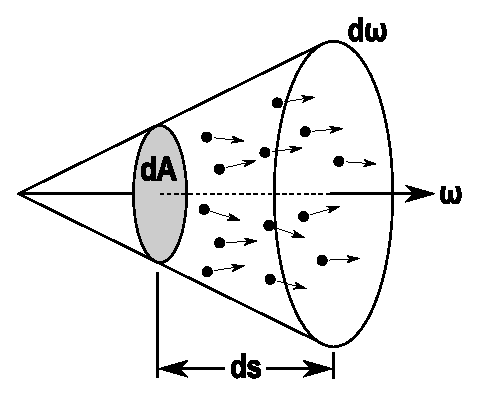
\includegraphics[height=0.3\textheight]{phasespacefluxsurface.eps}
		\caption{Teilchen, die das infinitesimale Fl"achenelement $d\location{A}$ durchqueren und sich in eine Richtung innerhalb des infinitesimalen Raumwinkelelements $d\omega$ um die Fl"achennormale $\omega$ von $d\location{A}$ bewegen.}
		\label{fig:phasespacefluxsurface}
	\end{figure}
	Der Phasenraumfluss ist ebenso wie die Phasenraumdichte eine fundamentale Gr"o"se, aus der wir alle anderen interessanten Gr"o"sen ableiten k"onnen. Im Folgenden werden wir uns aber meist auf den Phasenraumfluss beziehen.
		
	Unser Ziel ist es nun eine Bilanzgleichung f"ur die Teilchen in einem beliebigen Teil $V \times \Omega$ des Phasenraums (siehe Abb.~(\ref{fig:phasespacevolume})) aufzustellen. Dabei ist $V \subset \mathbb{R}^3$ ein Teilvolumen des $\mathbb{R}^3$ und $\Omega \subset \mathcal{S}^2$ ein beliebiger Raumwinkel aus der Einheitskugel $\mathcal{S}^2$. Dazu betrachten wir erst einmal die m"oglichen Gr"unde, die zu einer Ver"anderung der Teilchenzahl in unserem betrachteten Phasenraumvolumen $V \times \Omega$ f"uhren k"onnen.
	\begin{figure}
		\centering
		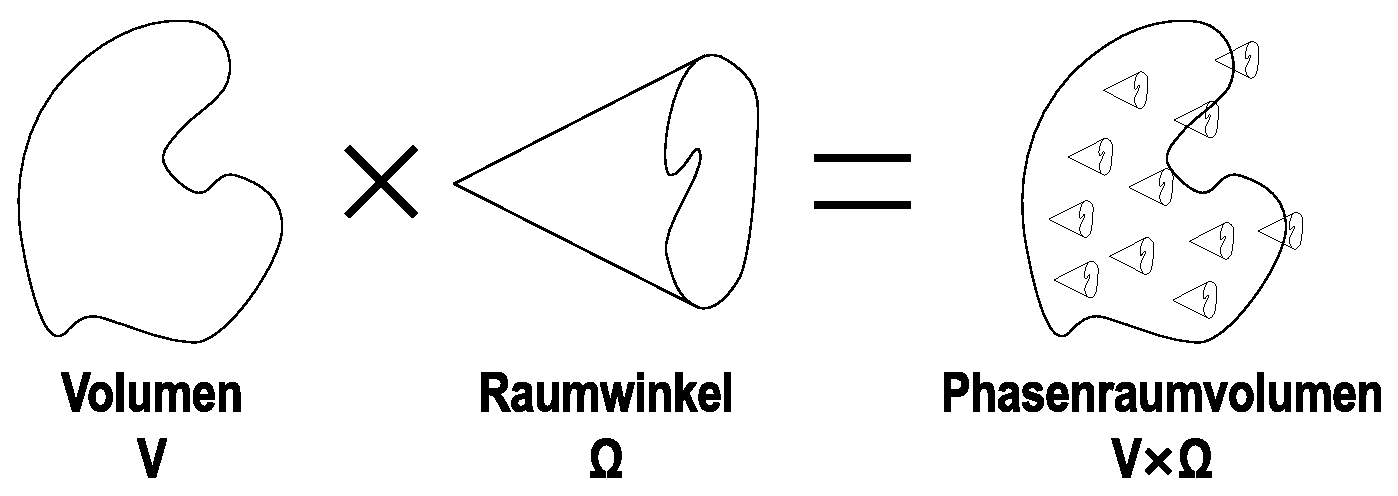
\includegraphics[width=0.8\textwidth]{phasespacevolume.eps}
		\caption{Darstellung einer Teilmenge $V \times \Omega$ des Phasenraums. Sie repr"asentiert alle Teilchen, die sich innerhalb des Volumens $V$ befinden und sich in eine Richtung innerhalb von $\Omega$ bewegen.}
		\label{fig:phasespacevolume}
	\end{figure}

	Zur {\em Emission} z"ahlt jeder Prozess, der neue Teilchen erzeugt. Dies kann durch verschiedene physikalische Prozesse wie z.B. chemische Reaktionen, thermische Emission oder Kernfusion begr"undet sein. Emission innerhalb von $V$ in eine Richtung innerhalb von $\Omega$ ver"andert also die Teilchenbilanz, da sie eine Quelle f"ur Teilchen darstellt. Nach der Emission bewegen sich die Teilchen in unserem Modell gradlinig mit konstanter Geschwindigkeit bis sie eine instantane Kollision mit dem Medium erfahren. Bewegt sich ein Teilchen bei seiner gradlinigen Bewegung in das Volumen $V$ hinein oder aus ihm heraus und bewegt es sich dabei in eine Richtung innerhalb von $\Omega$, so "andert dies ebenfalls unsere Teilchenbilanz. In diesem Fall sprechen wir von {\em Durchstr"omen}. Findet als letzte M"oglichkeit eine {\em Kollision} des Teilchens mit dem Medium innerhalb von $V$ statt, kann das Teilchen entweder absorbiert oder gestreut werden. Wird es absorbiert wirkt dies als Teilchensenke. Wird es gestreut, dann kann es, je nachdem in welche Richtung es sich vor und nach der Kollision bewegt hat, entweder keinen Einfluss auf die Teilchenbilanz haben (Bewegungsrichtung vor und nach der Kollision entweder innerhalb oder au"serhalb von $\Omega$), es kann herausgestreut werden (Bewegungsrichtung vor der Kollision innerhalb und nach der Kollision ausserhalb von $\Omega$) oder aber hineingestreut werden (Bewegungsrichtung vor der Kollision ausserhalb und nach der Kollision innerhalb von $\Omega$) werden.
	
	Um die einzelnen Beitr"age dieser Prozesse zur Teilchenbilanz quantitativ zu erfassen f"uhren wir die Teilchenzahl $$N(t):=\int_\Omega \int_V n(\location{r},\omega,t)\,d\location{r}\,d\omega$$ ein. Sie gibt an wieviele Teilchen sich zum Zeitpunkt $t$ im Phasenraumvolumen $V \times \Omega$ befinden. Durch die eben beschriebenen Prozesse "andert sich $N(t)$ normalerweise mit der Zeit. Ist die Zeit, die ein Teilchen ben"otigt das betrachtete System zu durchqueren, klein gegen"uber der typischen Zeitskala, nach der sich das System bedeutend ver"andert hat, k"onnen wir annehmen, dass sich die Teilchenzahl f"ur jedes Phasenraumvolumen im dynamischen Gleichgewicht befindet, d.h. dass zwar st"andig Teilchen aus dem Phasenraumvolumen hinein- und hinausstr"omen, erzeugt, absorbiert und gestreut werden, aber sich alle Prozesse in der Bilanz die Waage halten, $N(t)$ also station"ar ist:$$\frac{dN(t)}{dt}=0\qquad\left[\frac{1}{\text{s}}\right].$$ Teilen wir diese "Anderung von $N$ mit der Zeit auf die verschiedenen obengenannten Prozesse auf, sind wir bei der Grundlage einer Bilanzgleichung angelangt:$$\begin{bmatrix}\text{"Anderung}\\ \text{durch}\\ \text{Emission}\end{bmatrix}+\begin{bmatrix}\text{"Anderung}\\ \text{durch}\\ \text{Durchstr"omung}\end{bmatrix}+\begin{bmatrix}\text{"Anderung}\\ \text{durch}\\ \text{Kollisionen}\end{bmatrix}=0.$$ Wir leiten nun f"ur jeden dieser Ausdr"ucke einen Formelausdruck her.
	Die "Anderung aufgrund von Emission nennen wir $$\mathbf{E}=\int_\Omega \int_V q(\location{r},\omega)\,d\location{r}\,d\omega\qquad\left[\frac{1}{\text{s}}\right],$$ wobei wir die Phasenraumquellfunktion $q$ (mit Einheit $\text{m}^{-3}\text{sr}^{-1}\text{s}^{-1}$) eingef"uhrt haben, die f"ur jeden Ort $\location{r}$ und jede Raumrichtung $\omega$ die Anzahl erzeugter Teilchen pro Sekunde, Einheitsvolumen und Einheitsraumwinkel angibt. Hinein- und herausstr"omende Teilchen erzeugen eine Teilchenrate
	$$\mathbf{S}=\int_\Omega \int_{\partial V} \phi(\location{s},\omega)(\omega \cdot d\location{s})d\omega,$$
	die wir durch Integrieren "uber $\partial V$ (die Oberfl"ache von V) erhalten. Hierbei steht $\location{s}$ f"ur ein infinitesimales als Vektor repr"asentiertes Fl"achenelement, dessen Richtung die Fl"achennormale, und dessen L"ange seine Fl"ache repr"asentiert. Das Skalarprodukt zwischen Bewegungsrichtung $\omega$ und Fl"achennormalen sorgt f"ur das richtige Vorzeichen, wobei ein positiver Wert Teilchenverlust bedeutet.
	Der letzte Beitrag $\mathbf{C}$ tr"agt den Kollisionen Rechnung. Da Teilchen nur mit dem Medium, nicht aber untereinander interagieren, muss die Kollisionsrate unabh"angig von $\phi$ sein. Wir unterteilen $\mathbf{C}$ in einen Absorptionsteil $\mathbf{C}_\text{abs}$ und einen Streuanteil $\mathbf{C}_\text{sca}$. Wir nehmen an, dass die Wahrscheinlichkeit, dass ein Teilchen aufgrund von Absorption verschwindet proportional zur zur"uckgelegten Distanz im Medium, nicht aber von der Bewegungsrichtung durch das Medium ist (was gleichbedeutend mit der Annahme eines isotropen Mediums ist). Die Proportionalit"atskonstante am Ort $\location{r}$ nennen wir den (Volumen-)Absorptionsquerschnitt $\kappa(\location{r})$ ($[\kappa]=\frac{1}{\text{m}}=\frac{m^2}{m^3}$). Die zugeh"orige Teilchenrate ist
	$$\mathbf{C}_\text{abs}=\int_\Omega \int_V \kappa(\location{r})\phi(\location{r},\omega)\,d\location{r}\,d\omega.$$
	Die genauen Mechanismen der Streuung k"onnen durch Mie--Theorie oder Quantenmechanik behandelt werden. In unserem Teilchentransport repr"asentieren wir diese Streumodelle durch die Streuphasenfunktion $k(\location{r},\omega,\omega')$ und den Volumenstreuquerschnitt $\sigma(\location{r})$. Dabei gibt $k(\location{r},\omega,\omega')$ bei Streuung eines aus Richtung $\omega$ kommenden Teilchens am Ort $\location{r}$ die Wahrscheinlichkeit pro Einheitsraumwinkel an, nach $\omega'$ gestreut zu werden. Da ein gestreutes Teilchen irgendwohin gestreut wird, gilt f"ur $k$ die Normierungsbedingung
	\begin{equation}\label{eq:k_norm_req}
	  \int_{\mathcal{S}^2} k(\location{r},\omega,\omega')\,d\omega'=1.
	\end{equation}
	Au"serdem ist $k$ symmetrisch bez"uglich der Vertauschung der Bewegungsrichtungen vor und nach der Streuung:
	$$k(\location{r},\omega,\omega')=k(\location{r},\omega',\omega)\quad \forall\:\omega,\omega'\in\mathcal{S}^2.$$
	Beide Bedingungen werden z.B. durch die isotrope Streuphasenfunktion $$k_\text{iso}(\location{r},\omega,\omega')=\frac{1}{4\pi}$$ erf"ullt.
	Wie bei der Absorption, nehmen wir an, dass die Wahrscheinlichkeit eines Teilchens gestreut zu werden von der durch das Medium zur"uckgelegten Distanz, nicht aber von der Bewegungsrichtung abh"angt. Wir teilen $\mathbf{C}_\text{sca}$ weiter auf, in einen Teil
	$$\mathbf{C}_\text{out}=\int_\Omega \int_V \int_{\mathcal{S}^2} \sigma{(\location{r})}k(\location{r},\omega,\omega')\phi(\location{r},\omega)\,d\omega'\,d\location{r}\,d\omega,$$
	der herausgestreute Teilchen ber"ucksichtigt, sowie einen Teil
	$$\mathbf{C}_\text{in}=\int_\Omega \int_V \int_{\mathcal{S}^2} \sigma{(\location{r})}k(\location{r},\omega',\omega)\phi(\location{r},\omega')\,d\omega'\,d\location{r}\,d\omega$$
	entsprechend f"ur hineingestreute Teilchen. Dabei sollte erw"ahnt werden, dass sowohl $\mathbf{C}_\text{out}$ als auch $\mathbf{C}_\text{in}$ Teilchen ber"ucksichtigen, deren Richtung vor und nach der Streuung in $\Omega$ liegt, was weder einem Zuwachs noch einem Verlust an Teilchen entspricht. Da f"ur unsere Bilanz aber immer nur die Differenz von $\mathbf{C}_\text{out}$ und $\mathbf{C}_\text{in}$ betrachtet wird, hebt sich dieser Teil wieder heraus. Alternativ k"onnten wir auch "uber $\mathcal{S}^2 \setminus \Omega$ integrieren, was zu einer komplizierteren Rechnung, aber zu keinem anderen Endergebnis f"uhren w"urde. F"ugen wir die Einzelterme zusammen und ordnen nach Zuw"achsen und Verlusten sieht unsere Bilanzgleichung f"ur die Teilchenraten in $V \times \Omega$ wie folgt aus:
	$$\underbrace{\mathbf{S}+\mathbf{C}_\text{abs}+\mathbf{C}_\text{out}}_\text{Verluste}=\underbrace{\mathbf{E}+\mathbf{C}_\text{in}}_\text{Zuw"achse}$$
	Es f"allt bei der Betrachtung der Formeln f"ur die einzelnen Terme auf, dass alle Terme bis auf $\mathbf{S}$ Volumenintegrale "uber $V$ enthalten. $\mathbf{S}$ enth"alt stattdessen ein Oberfl"achenintegral "uber $\partial V$. Mithilfe des Gauss'schen Satzes dr"ucken wir das Oberfl"achenintegral "uber $\partial V$ durch ein Volumenintegral "uber $V$ aus und erhalten
	$$\mathbf{S}=\int_\Omega \int_V \omega \cdot (\nabla\phi)(\location{r},\omega)\,d\location{r}\,d\omega,$$
	wobei wir $\nabla \cdot(\omega\phi)=\omega\cdot(\nabla\phi)$ benutzt haben.
	
	In unserer Bilanzgleichung treten jetzt nur noch Volumenintegrale "uber unser Phasenraumvolumen $V \times \Omega$ auf. Da $V$ und $\Omega$ beliebig gew"ahlt waren, mu"s die Bilanzgleichung "uberall und in alle Richtungen lokale G"ultigkeit haben:
	\begin{multline*}
	  \omega\cdot\nabla\phi(\location{r},\omega)+\kappa(\location{r})\phi(\location{r},\omega)+\int_{\mathcal{S}^2}\sigma(\location{r})k(\location{r},\omega,\omega')\phi(\location{r},\omega)d\omega' \\
	  =q(\location{r},\omega)+\int_{\mathcal{S}^2}\sigma(\location{r})k(\location{r},\omega',\omega)\phi(\location{r},\omega')d\omega'
	\end{multline*}
	Da beim $\mathbf{C}_\text{out}$--Integral $\sigma$ und $\phi$ nicht von der Integrationsvariable abh"angen und das verbleibende Integral aufgrund der Normierungsbedingung (\ref{eq:k_norm_req}) gleich eins ist vereinfacht sich unsere Bilanzgleichung schlussendlich zu
	\begin{equation}\label{eq:particle_balance_equation}
	  \omega\cdot\nabla\phi(\location{r},\omega)+\left(\kappa(\location{r})+\sigma(\location{r})\right)\phi(\location{r},\omega)
	  =q(\location{r},\omega)+\sigma(\location{r})\int_{\mathcal{S}^2}k(\location{r},\omega',\omega)\phi(\location{r},\omega')d\omega'
	\end{equation}
	Die Bilanzgleichung hat die Gestalt einer Integro--Differentialgleichung in $\phi$.
	Im folgenden Abschnitt stellen wir den Bezug zwischen unseren abstrakten Teilchentransportgr"o"sen und physikalischen Strahlungsgr"o"sen her.

	\section{Ph"anomenologische Strahlungsgr"o"sen}\label{subsec:strahlungsgroessen}
	Im vorigen Abschnitt haben wir das Strahlungstransportproblem bewusst auf ein Teilchentransportproblem mit abstrakten Teilchen statt Photonen reduziert um einerseits eine klarere Herleitung zu erm"oglichen und um andererseits die Verwandtschaft zu anderen Transportproblemen (wie z.B. Neutronentransport) offensichtlich zu machen. Um nun den Anschluss zu radiometrischen Strahlungsgr"o"sen zu bekommen, ersetzen wir unsere abstrakten Teilchen wieder durch Photonen. Photonen haben zwei Eigenschaften die wir ber"ucksichtigen m"ussen. Sie bewegen sich konstant mit Lichtgeschwindigkeit, d.h. wir k"onnen die vorher gebrauchte allgemeine Teilchengeschwindigkeit $v$ gleich $\text{c}$ setzten. Au"serdem besitzt jedes Photon eine Energie, die durch seine Frequenz $\nu$ mit 
	$$E=h\nu \qquad[J]$$
	bestimmt ist. Dabei bezeichnet $h$ das Planck'sche Wirkungsquantum.
	Jeder Frequenz $\nu$ k"onnen wir ein monochromatisches Transportproblem zuordnen, dessen L"osung in Form eines Phasenraumflusses $\phi_\nu$ die Photonenfrequenz als Index tr"agt.
	Die {\em spezifische Intensit"at} $I_\nu(\location{r},\omega)$ erhalten wir nun aus dem Phasenraumfluss bzw. der Phasenraumdichte gem"a"s
	\begin{align}\label{eq:intensity_def}
		I_\nu(\location{r},\omega)d\nu & = h\nu\,\phi_\nu(\location{r},\omega)\\
		                       & = c h\nu\,n_\nu(\location{r},\omega) \qquad \left[\frac{\text{W}}{\text{m}^2\text{sr}}\right] \nonumber
	\end{align}
	Sie gibt an, wieviel Joule am Ort $\location{r}$ pro Sekunde durch eine Einheitsfl"ache mit Fl"achennormale $\omega$ pro Einheitsraumwinkel in Richtung $\omega$ und pro Frequenzintervall durch Photonen mit Frequenz $\nu$ transportiert wird:
	$$dE_\nu=I_\nu(\location{r},\omega) dA\,dt\,d\omega\,d\nu.$$
	Wir f"uhren au"serdem die {\em spezifische Emissivit"at} $\varepsilon_\nu$ ein. Wir erhalten Sie aus der Phasenraumquellfunktion $q_\nu$ durch
	\begin{equation}\label{eq:emissivity_def}
		\varepsilon_\nu(\location{r},\omega)d\nu = h\nu\,q_\nu(\location{r},\omega) \qquad \left[\frac{\text{W}}{\text{m}^3\text{sr}}\right].
	\end{equation}
	
	Multiplizieren wir unsere abstrakte Transportgleichung (\ref{eq:particle_balance_equation}) mit $h\nu$ und benutzen wir die Beziehungen (\ref{eq:intensity_def},\ref{eq:emissivity_def}) erhalten wir mit
	\begin{equation}\label{eq:stg_diff}
	  \omega\cdot\nabla I_\nu(\location{r},\omega)+\left(\kappa_\nu(\location{r})+\sigma_\nu(\location{r})\right)I_\nu(\location{r},\omega)
	  =\varepsilon_\nu(\location{r},\omega)+\sigma_\nu(\location{r})\int_{\mathcal{S}^2}k_\nu(\location{r},\omega',\omega)I_\nu(\location{r},\omega')d\omega'
	\end{equation}
	die {\em Strahlungstransportgleichung in differentieller Form}. Sie stellt eine Integro--Differentialgleichung f"ur $I_\nu$ auf unserem 5--dimensionalen Phasenraum $\mathbb{R}^3 \times \mathcal{S}^2$ dar und kann f"ur jede Frequenz $\nu$ getrennt gel"ost werden. Sie gibt f"ur jede Kombination aus Ort $\location{r}$ und Photonen--Ausbreitungsrichtung $\omega$ das lokal zu erf"ullende Gleichgewicht aus Verlusten (linke Seite) und Zuw"achsen (rechte Seite) an.
	
	Wir fassen die Verluste aufgrund von Absorption und Streuung durch den {\em Vo\-lu\-men\-ex\-tink\-ti\-ons\-quer\-schnitt}
	$$\xi_\nu(\location{r}):=\kappa_\nu(\location{r})+\sigma_\nu(\location{r}) \qquad\left[\frac{1}{m}\right]$$
	zusammen, wodurch wir (\ref{eq:stg_diff}) auch als
	\begin{equation}\label{eq:stg_diff2}
	  \omega\cdot\nabla I_\nu(\location{r},\omega)+\xi_\nu(\location{r})I_\nu(\location{r},\omega)
	  =\varepsilon_\nu(\location{r},\omega)+\sigma_\nu(\location{r})\int_{\mathcal{S}^2}k_\nu(\location{r},\omega',\omega)I_\nu(\location{r},\omega')d\omega'
	\end{equation}
	schreiben k"onnen.
	Au"serdem definieren wir die dimensionslose {\em optische Tiefe}
	\begin{equation*}
		\tau_\nu(\location{r}_1,\location{r}_2):=\int_{s=0}^{||\location{r}_2-\location{r}_1||} \xi_\nu(\location{r}_1+s(\location{r}_2 - \location{r}_1))\,ds,
	\end{equation*}
	die ein Ma"s f"ur die Undurchsichtigkeit des Mediums bei der Frequenz $\nu$ zwischen zwei Orten $\location{r}_1$ und $\location{r}_2$ ist. Nehmen wir uns Gleichung (\ref{eq:stg_diff2}), betrachten nur die Verluste (indem wir die rechte Seite zu Null setzen) und w"ahlen eine beliebige Richtung $\omega$, gelangen wir zur gew"ohnlichen Differentialgleichung
	$$I_\nu'(s)+\xi_\nu(s)I_\nu(s)=0,$$
	die durch
	\begin{equation}
		I_\nu(s)=I_\nu(0)\:\text{exp}\left(-\int_{s'=0}^s \xi_\nu(s')\right)=I_\nu(0)\:\text{exp}\left(-\tau_\nu(0,s)\right)
		\label{eq:exponentialdecay}
	\end{equation}
	gel"ost wird. Die L"osung zeigt, dass die optische Tiefe zu einer exponentiellen Abschw"achung der Intensit"at f"uhrt. Nach der Definition der verschiedenen ph"anomenologischen Strahlungsgr"o"sen schauen wir uns nun an, wie ihre Messung aufgefasst und mathematisch definiert werden kann.
	
	
	\section{Die Messgleichung}\label{sec:measurement_equation}
	Mit dem Strahlungsintensit"atsfeld, dass aus der Gesamtheit aller spezifischen Intensit"aten $I_\nu$ besteht, meinen wir die Funktion
	$$I:\mathbb{R}_+\times\mathbb{R}^3\times\mathcal{S}^2\to\mathbb{R}_+\;,\qquad (\nu,\location{r},\omega)\mapsto I_\nu(\location{r},\omega),$$
	die vom 6--dimensionalen Raum aller Photonenfrequenzen, Orte und Raumrichtungen auf die dort herrschende spezifische Intensit"at abbildet.
	
	Funktionen dieser Art bilden einen Skalarproduktraum. Das Null--Element ist die konstant auf Null abbildende Funktion. Zwei Funktionen lassen sich punktweise addieren und ergeben so eine neue Funktion, die auch nach $\mathbb{R}_{\geq 0}$ abbildet. Das Skalarprodukt zwischen zwei Funktionen $f$ und $g$ ist schlie"slich mit
	$$\langle f,g\rangle=\int_{\mathbb{R}_+} \int_{\mathbb{R}^3} \int_{\mathcal{S}^2} f(\nu,\location{r},\omega)g(\nu,\location{r},\omega)\,d\omega\,d\location{r}\,d\nu$$
	gegeben.
	
	Mit diesem funktionalanalytischen Handwerkszeug definieren wir eine Messung als das Skalarprodukt zwischen unserem Strahlungsintensit"atsfeld $I$ und einer {\em Sensitivit"atsfunktion} $W$, welche die St"arke der Gewichtung angibt, mit der die spezifische Intensit"at der Frequenz $\nu$ am Ort $\location{r}$ in Richtung $\omega$ in den Messwert eingeht. Die entsprechende Formel
	\begin{equation}\label{eq:messgleichung}
		M^{(i)}:=\langle W^{(i)},I\rangle=\int_{\mathbb{R}_+} \int_{\mathbb{R}^3} \int_{\mathcal{S}^2} W^{(i)}(\nu,\location{r},\omega)I_\nu(\location{r},\omega)\,d\omega\,d\location{r}\,d\nu
	\end{equation}
	nennen wir {\em Messgleichung} (f"ur den $i$--ten Sensor). F"ur monochromatische Messungen f"uhren wir zus"atzlich noch 
	\begin{equation}\label{eq:messgleichung_mono}
		M_\nu^{(i)}:=\langle W_\nu^{(i)},I_\nu\rangle=\int_{\mathbb{R}^3} \int_{\mathcal{S}^2} W_\nu^{(i)}(\location{r},\omega)I_\nu(\location{r},\omega)\,d\omega\,d\location{r}
	\end{equation}
	ein, womit wir (\ref{eq:messgleichung}) auch als
	\begin{equation}\label{eq:messgleichung_frommonos}
		M^{(i)}=\int_{\mathbb{R}_+} M_\nu^{(i)}\,d\nu
	\end{equation}
	schreiben k"onnen.
	Die Tatsache, dass wir die Sensitivit"atsfunktion nicht n"aher spezifizieren, erlaubt uns die gr"o"stm"ogliche Freiheit beim kreieren virtueller Sensoren. Beispielsweise k"onnte $W$ nur in einem kleinen Volumen und einem kleinen Raumwinkel, aber bei allen Frequenzen, nichtverschwindend sein, und so einen virtuellen Sensor zur Messung der Gesamt--Intensit"at an einem bestimmten Ort in eine bestimmte Richtung repr"asentieren. Ebenso kann durch gleichstarke Gewichtung aller Raumrichtungen die mittlere Intensit"at gemessen werden.
	
	Was hier vielleicht als ein nur theoretisch interessantes Konstrukt ohne praktischen Nutzen erscheint, erweist sich sp"ater insbesondere in Verbindung mit Monte--Carlo--Sampling als ein gleichzeitig vielseitiges und effizientes Werkzeug.	
	
	
	\section{"Ubersicht etablierter L"osungsverfahren}
	TODO: "Ubersicht benutzter L"osungsverfahren, Meilensteine (wann zum ersten mal Polarisation gerechnet?, Warum etablieren sich MC-Verfahren so sp"at?, etc...)
		
	\chapter{Pfadintegralformulierung der Strahlungstransportgleichung}\label{chapter:path_radiative_transfer}
	In diesem Abschnitt leiten wir eine alternative mathematische Formulierung der Strahlungstransportgleichung einerseits und ihrer L"osung (genau genommen, Messungen der L"osung im Sinne von (\ref{eq:messgleichung})) andererseits her. Dies f"uhrt uns durch die verschiedenen auf das Problem eingenommenen Blickwinkel zu einem besseren Verst"andnis von Strahlungstransport und gibt uns dar"uber hinaus einen neuen Ansatzpunkt zur effizienten L"osung des Strahlungstransportproblems.
	
	Die Idee zu dieser Formulierung kommt aus der Dissertation von \citet{Veach:1997p9136}, wird aber schon in \citep{Arvo:1995p9257} vorgestellt. Beide Dissertationen behandeln allerdings nur den Strahlungstransport zwischen Oberfl"achen. In der Arbeit von \citet{Pauly:2000p5705} wird dies auf partizipierende Medien ausgedehnt. Aus \citep{Arvo:1993p9035} stammt au"serdem die Herleitung der integralen Form der Strahlungstransportgleichung.
	
	
	\section{Strahlungstransportgleichung in integraler Form}
	In differentieller Form nimmt die Strahlungstransportgleichung, wie wir in Abschnitt (\ref{subsec:strahlungsgroessen}) gesehen haben, folgende Gestalt an:
		\begin{equation}
			\omega \cdot \nabla I(\location{r},\omega)+\overbrace{\left(\kappa(\location{r})+\sigma(\location{r})\right)}^{=:\xi(\location{r})}I(\location{r},\omega)=\varepsilon(\location{r},\omega)+\sigma(\location{r}) \int_{\mathcal{S}^2} k(\location{r},\omega',\omega)I(\location{r},\omega') d\omega'.
			\label{eq:diff.STG}
		\end{equation}
	F"ur diesen und die folgenden Abschnitte lassen wir dabei den Index $\nu$ aus "Ubersichtsgr"unden weg, womit gemeint ist, dass wir stellvertretend f"ur alle Frequenzen ein einzelnes monochromatisches Strahlungstransportproblem einer beliebigen Frequenz nehmen. Wenn wir zum polychromatischen Fall zur"uckkehren f"uhren wir die Indizes wieder ein.
	
	Schreiben wir das Skalarprodukt zwischen $\omega$ und dem $\nabla$--Operator als Richtungsableitung
	\newcommand{\dds}{\frac{\text{d}}{\text{d}s}}
	\newcommand{\ddszero}{\left. \dds \right|_{s=0}}
	\begin{equation*}
		\omega \cdot \nabla I(\location{r},\omega)
		=  \ddszero I(\location{r}+s\,\omega,\omega)
		=  -\ddszero I(\location{r}-s\,\omega,\omega)
	\end{equation*}
	k"onnen wir (\ref{eq:diff.STG}) als
	\begin{multline}
		\dds I(\location{r}-s\,\omega,\omega) - \xi(\location{r}-s\,\omega)I(\location{r}-s\,\omega,\omega) = \\-\varepsilon(\location{r}-s\,\omega,\omega) -\sigma(\location{r}-s\,\omega) \int_{\mathcal{S}^2} k(\location{r}-s\,\omega,\omega',\omega)I(\location{r}-s\,\omega,\omega') \text{d}\omega'
		\label{eq:diff.STGtranslated}
	\end{multline}
	umschreiben. Dabei haben wir die Beschr"ankung $s=0$ fallengelassen, was die Korrektheit der Umformung aber nicht "andert. Mit den Abk"urzungen
	\begin{align*}
		{\hat I}(s)&:=I(\location{r}-s\,\omega,\omega) \\
		Q(\location{r},\omega)&:= \varepsilon(\location{r},\omega)+\sigma(\location{r}) \int_{\mathcal{S}^2} k(\location{r},\omega',\omega)I(\location{r},\omega') d\omega' \\
		{\hat Q}(s)&:=Q(\location{r}-s\,\omega,\omega)\\
		{\hat \xi}(s)&:=\xi(\location{r}-s\,\omega) \\
		{\hat \tau}(s)&:= \int_{s'=0}^{s} {\hat \xi}(s') \text{d}s'
	\end{align*}
	wird aus (\ref{eq:diff.STGtranslated})
	\begin{equation}
		\dds {\hat I}(s) - {\hat \xi}(s){\hat I}(s)= -{\hat Q}(s) \qquad |\cdot e^{-{\hat \tau}(s)}.
		\label{eq:diff.STGhatted}
	\end{equation}
	Gleichung (\ref{eq:diff.STGhatted}) ist eine gew"ohnliche Differentialgleichung die sich mit
	\begin{align}
		(\ref{eq:diff.STGhatted})\Leftrightarrow\qquad \dds \left(e^{-{\hat \tau}(s)} {\hat I}(s)\right)&= -e^{-{\hat \tau}(s)} {\hat Q}(s) \qquad | \int_{s'=0}^s (\cdot)\text{d}s' \nonumber \\
		\Leftrightarrow\qquad e^{-{\hat \tau}(s)} {\hat I}(s) - {\hat I}(0) &= -\int_{s'=0}^s e^{-{\hat \tau}(s')} {\hat Q}(s') \text{d}s' \nonumber \\
		\Leftrightarrow\qquad {\hat I}(0) &= e^{-{\hat \tau}(s)} {\hat I}(s) + \int_{s'=0}^s e^{-{\hat \tau}(s')} {\hat Q}(s') \text{d}s' \label{eq:diff.STGpreintegral}
	\end{align}
	leicht nach ${\hat I}(0)$ aufl"osen l"asst. Obwohl ${\hat Q}(s)$ lokal die Intensit"at $I$ "uber alle Raumrichtungen integriert, d"urfen wir f"ur die L"osung von (\ref{eq:diff.STGhatted}) $Q$ als unabh"angig von $I$ behandeln, da die Schnittmenge zwischen der Geraden im Raum, auf der wir die Differentialgleichung l"osen, und der Menge aller Raumrichtungen $\mathcal{S}^2$ bei der Integration "uber alle Raumrichtungen eine Nullmenge ist und somit f"ur physikalisch relevante Strahlungsintensit"atsfelder (d.h. solche, die hinreichend stetig/beschr"ankt bzw. keine Delta--Distribution sind) keinen Beitrag zum Integral leistet.
	Setzen wir in (\ref{eq:diff.STGpreintegral}) f"ur die Abk"urzungen wieder die urspr"unglichen Ausdr"ucke ein, erhalten wir die {\em Strahlungstransportgleichung in integraler Form}:
	\begin{multline}
		I(\location{r},\omega) = e^{-\tau(\location{r},\location{r}-s\,\omega)} {\hat I}(\location{r},\location{r}-s\,\omega) + \int_{s'=0}^\infty e^{-\tau(\location{r},\location{r}-s\,\omega)} \;\cdot \\
		\quad\cdot\left( \varepsilon(\location{r}-s'\,\omega,\omega) + \sigma(\location{r}-s'\,\omega)
		\left[ \int_{\mathcal{S}^2} k(\location{r}-s'\,\omega,\omega',\omega)I(\location{r}-s'\,\omega,\omega') \text{d}\omega'\right] \right) \text{d}s'
		\label{eq:int.STG}
	\end{multline}
	Nehmen wir nun als Randbedingungen an, dass in unendlich gro"ser Entfernung keine Lichtquellen existieren, d.h. $\forall \omega \in \mathcal{S}^2 : I(\location{r}=-\infty\cdot\omega,\omega)=0$, dann vereinfacht sich (\ref{eq:int.STG}) zu
	\begin{multline}
		I(\location{r},\omega) = \int_{s'=0}^\infty e^{-\tau(\location{r},\location{r}-s\,\omega)} \;\cdot \\
		\quad\cdot\left( \varepsilon(\location{r}-s'\,\omega,\omega) + \sigma(\location{r}-s'\,\omega)
		\left[ \int_{\mathcal{S}^2} k(\location{r}-s'\,\omega,\omega',\omega)I(\location{r}-s'\,\omega,\omega') \text{d}\omega'\right] \right) \text{d}s'
		\label{eq:int.STGdarkbg}
	\end{multline}


	\section{Strahlungstransportgleichung in Operator--Form}
	Schauen wir uns die einzelnen Teile der Gleichung (\ref{eq:int.STGdarkbg}) genauer an.
	Der innere Teil von (\ref{eq:int.STGdarkbg}) in eckigen Klammern summiert an einem festen Ort ($\location{r}-s'\,\omega$), mit der Streuphasenfunktion $k$ gewichtet, die einfallenden Intensit"aten auf, die in Richtung $\omega$ gestreut werden. Anschlie"send skaliert der Volumenstreuquerschnitt die aufintegrierte Intensit"at entsprechend dem lokal vorhandenen Medium und gibt dabei dem Ausdruck die Einheit einer Emissivit"at.
	Der restliche "au"sere Teil der Gleichung addiert die eben gewonnene Emissivit"at durch Einstreuung zu der lokal durch Ausstrahlung erzeugten Emissivit"at an jedem Punkt auf einer Geraden hinter dem Punkt $\location{r}$ und summiert die mit einem der optischen Tiefe entsprechenden Abschw"achungsfaktor gewichteten, in Richtung $\omega$ zeigenden, Emissivit"aten, entlang der Geraden zur Gesamtintensit"at am Ort $\location{r}$ in Richtung $\omega$ auf.
	Der Gesamtausdruck l"asst sich durch Einf"uhrung zweier neuer Operatoren
	\begin{align*}
		\left(\mathbf{G}\varepsilon\right)(\location{r},\omega)&:=\int_{s'=0}^\infty e^{-\tau(\location{r}-s' \omega,\location{r})}\varepsilon(\location{r}-s' \omega,\omega) ds' \\
		\left(\mathbf{K}I\right)(\location{r},\omega)&:=\sigma(\location{r})\int_{S^2} k(\location{r},\omega',\omega) I(\location{r},\omega') d\omega'
	\end{align*}
	\begin{equation*}
		\mathbf{G} : \varepsilon(\location{r},\omega) \mapsto I(\location{r},\omega) , \qquad
		\mathbf{K} : I(\location{r},\omega) \mapsto \varepsilon(\location{r},\omega)
	\end{equation*}
	in elementarere Prozesse aufteilen. Wir nennen $\mathbf{G}$ den sogenannten {\em Fortpflanzungs--Operator} und $\mathbf{K}$ den {\em Streu--Operator}. Beides sind Integraloperatoren auf dem Raum der Funktionen $f : \mathbb{R}^3 \times \mathcal{S}^2 \to \mathbb{R}_+$, die vom Teilchen--Phasenraum auf die positiven reellen Zahlen abbilden. Beide haben komplement"are Lokalit"aten. W"ahrend $\mathbf{K}$ lokal im Ort "uber alle Raumrichtungen integriert, ist $\mathbf{G}$ lokal in der Raumrichtung und integriert "uber alle Orte entlang einer Geraden im Raum. Dabei bildet $\mathbf{K}$ von einem Strahlungsintensit"atsfeld auf ein Emissivit"atsfeld ab. Bei $\mathbf{G}$ ist es umgekehrt, es macht aus einem Emissivit"atsfeld wieder ein Strahlungsintensit"atsfeld.
	Mit diesen neuen Operatoren wird aus Gleichung (\ref{eq:int.STGdarkbg}) die {\em Operatorform der Strahlungstransportgleichung}
	\begin{equation}
		I=\mathbf{G}(\varepsilon + \mathbf{K}I),
		\label{eq:op.STG}
	\end{equation}
	die wir nach $I$ aufl"osen k"onnen:
	\begin{align}
		(\ref{eq:op.STG}) \Leftrightarrow I&=\mathbf{G}\varepsilon + \mathbf{GK}I \nonumber \\
		\Leftrightarrow (\mathbf{1}-\mathbf{GK})I &= \mathbf{G}\varepsilon \nonumber \\
		\Leftrightarrow I &= (\mathbf{1}-\mathbf{GK})^{-1}\mathbf{G}\varepsilon \label{eq:op.STGinvert} \\
		\Leftrightarrow I &= \sum_{k=0}^\infty (\mathbf{GK})^k \mathbf{G}\varepsilon \label{eq:op.STGneumann} \\
		&=\mathbf{G}\varepsilon + \mathbf{GKG}\varepsilon + \mathbf{GKGKG}\varepsilon + \hdots \label{eq:op.STGneumann.explicit} \\
		\Leftrightarrow I &=\sum_{k=0}^\infty \mathbf{G} (\mathbf{KG})^k \varepsilon \label{eq:op.STGkg}
	\end{align}
	Damit ist das Strahlungstransportproblem formal gel"ost! Dabei haben wir den auftretenden invertierten Operator (\ref{eq:op.STGinvert}) durch eine Neumann--Reihe (\ref{eq:op.STGneumann}) ersetzt. Dies ist dann zul"assig wenn die Operatornorm des Operators $\mathbf{GK}$ kleiner als eins ist und damit sichergestellt ist, dass die Neumann--Reihe konvergiert. F"ur alle praktisch relevanten Probleme ist dies der Fall \citep[siehe][Theorem 12 und 13]{Arvo:1995p9257}. Physikalisch l"asst sich das Gleichgewichts--Strahlungsintensit"atsfeld als Summe aus Intensit"atsfeldern verstehen, die durch Photonen mit unterschiedlich vielen Streuereignissen auf ihrem Weg von der Emission aus einer Lichtquelle bis zu ihrer Messung mit einem Messinstrument entstanden sind (wie in Schritt (\ref{eq:op.STGneumann.explicit}) deutlich wird). Dabei m"ussen Pfade jeder m"oglichen L"ange (sprich Anzahl an Streuereignissen) ber"ucksichtigt werden. Zwischen Emission und Messung wechseln sich dabei Fortpflanzung $\mathbf{G}$ und Streuung $\mathbf{K}$ ab. Im letzen Schritt (\ref{eq:op.STGkg}) haben wir $\mathbf{G}$ nach links ausgeklammert um den $\mathbf{KG}$--Operator herauszustellen.
	
	
	\section{KG--Operator in Volumenform}
	Schauen wir uns den $\mathbf{KG}$--Operator genauer an. Nachdem $\mathbf{KG}$ ein Emissivit"atsfeld durch Fortpflanzung zu einem Intensit"atsfeld aufintegriert hat, wird dieses durch die anschliessende Streuung erneut auf ein Emissivit"atsfeld abgebildet:
	\begin{equation*}
		\mathbf{KG} : \varepsilon(\location{r},\omega) \mapsto \varepsilon(\location{r},\omega)
	\end{equation*}

	Setzen wir die Definitionen der Operatoren ein und fassen die Integrale zusammen:
	\begin{align*}
		\left(\mathbf{KG}\varepsilon\right)(\location{r},\omega)&=\sigma(\location{r}) \int_{\mathcal{S}^2} k(\location{r},\omega',\omega)\left[\int_{s'=0}^\infty e^{-\tau(\location{r}-s' \omega',\location{r})}\varepsilon(\location{r}-s' \omega',\omega') \text{d}s'\right] \text{d}\omega' \\
		&=\sigma(\location{r}) \int_{\mathcal{S}^2} \int_{s'=0}^\infty k(\location{r},\omega',\omega) e^{-\tau(\location{r}-s' \omega',\location{r})}\varepsilon(\location{r}-s' \omega',\omega') \underbrace{\text{d}s' \text{d}\omega'}_{=\frac{\text{d}\location{r}'}{s'^2}} \\
		&=\sigma(\location{r}) \int_{\mathbb{R}^3} k(\location{r},\omega',\omega) \frac{e^{-\tau(\location{r}',\location{r})}}{\|\location{r}-\location{r}'\|^2}\varepsilon(\location{r}',\omega') \,\text{d}\location{r}'
	\end{align*}
	Da wir durch Kombination der Integration "uber alle Raumrichtungen $\omega'$ und alle Entfernungen $s'$ den gesamten Raum abdecken, k"onnen wir die beiden Integrale zugunsten eines Volumenintegrals "uber den gesamten Raum sowie eines geometrischen Verd"unnungsfaktors tauschen. Mit dem Ziel, sp"ater alle Integrationen zu Volumenintegralen zusammenzufassen, schreiben wir den $\mathbf{KG}$--Operator so um, dass alle expliziten Angaben von Entfernungen und Raumrichtungen durch eine raumpunktorientierte Notation ersetzt werden:
	\begin{multline}
		\left(\mathbf{KG}\varepsilon\right)(\location{r}_i \rightarrow\location{r}_{i+1})=\\
		\sigma(\location{r}_i) \int_{\mathbb{R}^3} k(\location{r}_{i-1}\rightarrow\location{r}_i\rightarrow\location{r}_{i+1})\frac{e^{-\tau(\location{r}_{i-1},\location{r}_i)}}{\|\location{r}_i-\location{r}_{i-1}\|^2}\varepsilon(\location{r}_{i-1} \rightarrow\location{r}_i)d\location{r}_{i-1}
		\label{eq:KGvolume_intermediate}
	\end{multline}
	Wir f"uhren zus"atzlich noch die Abk"urzung
	\begin{align*}
		\scatter{i}\;&:=\sigma(\location{r}_i)k(\location{r}_{i-1}\rightarrow\location{r}_i\rightarrow\location{r}_{i+1})\\
			&=\sigma(\location{r}_i)k(\location{r}_i,\normalized{\location{r}_i-\location{r}_{i-1}},\normalized{\location{r}_{i+1}-\location{r}_i})
	\end{align*}
	ein, so dass wir (\ref{eq:KGvolume_intermediate}) zusammen mit den in Abschnitt \ref{subsec:nomenklatur} eingef"uhrten Schreibweisen noch kompakter als
	\begin{equation}
		\left(\mathbf{KG}\varepsilon\right)_{(i,i+1)}=\int_{\mathbb{R}^3} \scatter{i}\frac{e^{-\tau_{(i-1,i)}}}{d_{(i-1,i)}^2}\varepsilon_{(i-1,i)}d\location{r}_{i-1}.
		\label{eq:KGvolume}
	\end{equation}
	schreiben k"onnen.


	\section{Pfadintegrall"osung der Strahlungstransportgleichung}
	Wir setzen die Neumann--Reihen--L"osung (\ref{eq:op.STGkg}) in die monochromatische Me"sgleichung (\ref{eq:messgleichung_mono}) ein und erhalten
	\begin{align}
		M_\nu&=\int_{\mathbb{R}^3}\int_{\mathcal{S}^2}W_\nu(\location{r},\omega) \left(\sum_{k=0}^\infty \mathbf{G} (\mathbf{KG})^k \varepsilon_\nu\right)(\location{r},\omega) \,\text{d}\omega \,\text{d}\location{r} \nonumber \\
		&=\sum_{k=0}^\infty \int_{\mathbb{R}^3}\int_{\mathcal{S}^2}W_\nu(\location{r},\omega) \left(\mathbf{G} (\mathbf{KG})^k \varepsilon_\nu\right)(\location{r},\omega) \,\text{d}\omega \,\text{d}\location{r} \nonumber \\
		&=\sum_{k=0}^\infty \int_{\mathbb{R}^3}\int_{\mathcal{S}^2}W_\nu(\location{r},\omega) \int_{s'=0}^\infty e^{-\tau_\nu(\location{r}-s' \omega,\location{r})} \left((\mathbf{KG})^k \varepsilon_\nu\right)(\location{r},\omega) \underbrace{\text{d}s' \,\text{d}\omega}_{=\frac{\text{d}\location{r}'}{s'^2}} \,\text{d}\location{r} \nonumber \\
		&=\sum_{k=0}^\infty \int_{\mathbb{R}^3}\int_{\mathbb{R}^3}W_\nu(\location{r}'\rightarrow\location{r}) \frac{e^{-\tau_\nu(\location{r}',\location{r})}}{\|\location{r}'-\location{r}\|^2} \left((\mathbf{KG})^k \varepsilon_\nu\right)(\location{r}'\rightarrow\location{r}) \,\text{d}\location{r}' \,\text{d}\location{r}.
		\label{eq:STGprepathsolution}
	\end{align}
	Durch rekursives Einsetzen von (\ref{eq:KGvolume}) in (\ref{eq:STGprepathsolution}) und Neuanordnung der Terme erhalten wir dann als Ergebnis einer monochromatischen Messung:
	\begin{equation}
		M_\nu=\sum_{k=0}^\infty \underbrace{\idotsint}_{(k+2)\text{--mal}}\varepsilon_{\nu,(0,1)}\left[\prod_{i=1}^k\frac{e^{-\tau_{\nu,(i-1,i)}}}{d_{(i-1,i)}^2}\scatter{i}\right]\frac{e^{-\tau_{\nu,(k,k+1)}}}{d_{(k,k+1)}^2} W_{\nu,(k,k+1)} \;\text{d}\location{r}_0 \dotsm \text{d}\location{r}_{k+1} .
		\label{eq:STGpathsolution}
	\end{equation}
	Das Ergebnis ist eine Summe aus reinen $(k+2)$--fachen Volumenintegralen "uber den ganzen Raum, wobei "uber den m"oglichen Start- und Endpunkt sowie die $k$ Streupunkte innerhalb des Photonenpfades integriert wird.
	Anschaulich m"ussen wir also die Beitr"age von Pfaden jeder Anzahl an Streupunkten und jeder m"oglichen Anordnung von Emissions-, Streu- und Mess\-orten aufsummieren. Dies wird vielleicht klarer, wenn wir die ersten Terme der Summe explizit ausformulieren:
	\begin{align*}
		M_\nu&=\iint_{(\mathbb{R}^3)^2}\varepsilon_{\nu,(0,1)}\frac{e^{-\tau_{\nu,(0,1)}}}{d_{(0,1)}^2} W_{\nu,(0,1)} \;\text{d}\location{r}_0\text{d}\location{r}_1 \\
		&+\iiint_{(\mathbb{R}^3)^3}\varepsilon_{\nu,(0,1)}\frac{e^{-\tau_{\nu,(0,1)}}}{d_{(0,1)}^2}\scatter{1}\frac{e^{-\tau_{\nu,(1,2)}}}{d_{(1,2)}^2} W_{\nu,(1,2)} \;\text{d}\location{r}_0\text{d}\location{r}_1\text{d}\location{r}_2 \\
		&+\iiiint_{(\mathbb{R}^3)^4}\varepsilon_{\nu,(0,1)}\frac{e^{-\tau_{\nu,(0,1)}}}{d_{(0,1)}^2}\scatter{1}\frac{e^{-\tau_{\nu,(1,2)}}}{d_{(1,2)}^2}\scatter{2}\frac{e^{-\tau_{\nu,(2,3)}}}{d_{(2,3)}^2} W_{\nu,(2,3)} \;\text{d}\location{r}_0\text{d}\location{r}_1\text{d}\location{r}_2\text{d}\location{r}_3 \\
		&+\hdots
	\end{align*}
	Diese Form der L"osung des Strahlungstransportproblems hat mehrere Vorteile:
	\begin{itemize}
		\item{Die L"osung besitzt eine anschauliche Interpretation}
		\item{Die L"osung ist explizit, es muss keine implizite Integro--Differentialgleichung wie (\ref{eq:stg_diff}) gel"ost werden}
		\item{Die L"osung ist ein reines Integrationsproblem und somit ein gutes Gegenst"uck zu hochdimensionalen Monte--Carlo--Integrations--Verfahren, wie wir in Abschnitt \ref{subsec:integrationsproblem_comparison} sehen werden}
	\end{itemize}
	Das polychromatische Messergebnis ergibt sich nun einfach durch Einsetzen von (\ref{eq:STGpathsolution}) in (\ref{eq:messgleichung_frommonos}).


	\section{Elimination der Neumann--Reihe}\label{sec:neumann_elimination}
	Unsere Darstellung der L"osung (\ref{eq:STGpathsolution}) des Strahlungstransportproblems besteht bisher aus einer unendlichen Summe von Integralen, was eine direkte Folge der Aufspaltung des L"osungsoperators aus (\ref{eq:op.STGinvert}) in seine Neumann--Reihe (\ref{eq:op.STGneumann}) ist. In dieser Form sind die Pfade in Klassen gleicher L"ange (d.h. Anzahl an Streupunkten) eingeteilt, was die mathematische Behandlung vereinfacht, da die F"alle verschiedener L"ange getrennt voneinander behandelt werden k"onnen. Gleichzeitig verleitet diese Darstellung jedoch dazu zu glauben, es w"are sinnvoll oder l"age in der Natur der Sache, die Pfade unterschiedlicher L"ange getrennt voneinander zu behandeln. Tats"achlich gibt es aber keinen physikalischen Grund daf"ur, vielmehr w"are es auch mathematisch hilfreich die L"osung als ein einziges Integral "uber den Raum aller Pfade darzustellen, da wir es dann formal mit nur noch einem Integrationsproblem zu tun h"atten und nicht mehr mit unendlich vielen.
	
	Daher f"uhren wir nun \citet[][8.2]{Veach:1997p9136} folgend, die Menge aller Pfade sowie ein passendes Integrationsma"s ein, um unsere L"osung (\ref{eq:STGpathsolution}) als Einzelintegral darstellen zu k"onnen. Sei dazu $\Omega_{\nu,k}$ die Menge aller Pfade der Frequenz $\nu$ und der L"ange $k$, d.h. Pfade der Form
	$${\overline x}=\location{r}_0\location{r}_1\cdots\location{r}_k\location{r}_{k+1},$$
	mit $k\in\{0,1,2,\dots\}$ und $\location{r}_i \in \mathbb{R}^3$ f"ur alle $i$. Wir definieren mittels
	$$\mu_k(D)=\int_D d\nu d\location{r}_0\cdots d\location{r}_{k+1}$$
	ein Ma"s f"ur Pfade der L"ange $k$, wobei $D\subset\Omega_k$ eine Teilmenge von Pfaden dieser L"ange repr"asentiert und $d\location{r}_i$ das geometrische Volumenma"s sowie $d\nu$ das Integrationsma"s "uber die positiven reellen Zahlen darstellt. Der Raum aller Pfade ist die Vereinigung
	$$\Omega=\bigcup_{k=0}^\infty \Omega_k$$
	der Mengen von Pfaden verschiedener L"angen. Da"s Ma"s f"ur die Integration von beliebigen Teilmengen des Pfadraumes $D\subset\Omega$ ist nun durch
	$$\mu(D)=\sum_{k=0}^\infty \mu_k(D\cap\Omega_k)$$
	gegeben, d.h. das Ma"s f"ur $D$ ist einfach die Summe der Ma"se von Pfaden aus $D$ entsprechender L"ange. Benennen wir nun noch den pfadl"angen- und frequenzabh"angigen Integranden aus (\ref{eq:STGpathsolution})
	\begin{equation}
		f({\overline x}_\nu)=f_\nu(\location{r}_0\location{r}_1\cdots\location{r}_k\location{r}_{k+1})=\varepsilon_{\nu,(0,1)}\left[\prod_{i=1}^k\frac{e^{-\tau_{\nu,(i-1,i)}}}{d_{(i-1,i)}^2}\scatter{i}\right]\frac{e^{-\tau_{\nu,(k,k+1)}}}{d_{(k,k+1)}^2} W_{\nu,(k,k+1)}
		\label{eq:mcf}
	\end{equation}
	als {\em Messbeitragsfunktion} $f$, dann k"onnen wir nun die polychromatische Messung (\ref{eq:messgleichung}) einfach als
	\begin{equation}
		M=\int_\Omega f({\overline x})d\mu({\overline x})
		\label{eq:unified_measurementintegral}
	\end{equation}
	schreiben. Es ist in dieser Form leichter einzusehen, dass wir die Pfade nicht nach ihrer L"ange zusammengefasst behandeln m"ussen, um anschlie"send die (unendlich vielen) Ergebnisse aufzusummieren, sondern stattdessen Pfade in beliebiger Weise zur Integration zusammenfassen d"urfen. Dies ist insbesondere f"ur die Monte--Carlo--Integration wichtig, da unsere ganze Theorie sich dort auf die L"osung eines Einzelintegrals beschr"anken wird und wir dadurch dort nahtlos mit der L"osung von Messintegralen der Form (\ref{eq:unified_measurementintegral}) ankn"upfen k"onnen.

		\chapter{Monte--Carlo--Integration}\label{chapter:mc_integration}
	Monte--Carlo--Verfahren liegt die Idee zugrunde, zu einem numerischen Problem ein passendes Zufallsexperiment so zu konstruieren, so dass der Erwartungswert einer Zufallsvariable des Experiments das numerische Problem löst.
	
	Die Idee ist nicht neu, so fÜhrte {\em Buffon} 1777 folgendes Experiment durch: Eine Nadel der LÄnge $L$ wird wiederholt auf eine plane FlÄche mit parallelen Linien im Abstand $d>L$ fallengelassen und jeweils notiert, ob die Nadel eine der Linien kreuzt. Er zeigte, dass der Erwartungswert fÜr die Wahrscheinlichkeit der Nadel, die Linie zu kreuzen $$p=\frac{2L}{\pi d}$$ betrÄgt. Laplace wies spÄter darauf hin, dass  man die HÄufigkeit, mit der die Nadeln die Linien kreuzen, auch Nutzen kann, um den Wert von $\pi$ zu schÄtzen (siehe Abb. \ref{fig:buffon}): $$\pi=\frac{2L}{p d}\approx \frac{2L}{\frac{k}{N}d}$$
	(\text{N Experimente, davon k mal eine Linie gekreuzt}).
	\begin{figure}
		\centering
		\includegraphics[height=0.3\textheight]{buffonsneedles.eps}
		\caption{Beispiel fÜr eine Realisierung des Buffon--Nadel--Experiments mit 100 geworfenen Nadeln. Der erhaltene SchÄtzwert fÜr $\pi$ ist bei so wenigen Nadeln nicht sehr genau.}
		\label{fig:buffon}
	\end{figure}
	
	\section{Das Integrationsproblem}\label{subsec:integrationsproblem}
	Betrachten wir das Integral
	\begin{equation}
		I=\int_\Omega f(x) d\mu(x),
		\label{eq:integration_problem}
	\end{equation}
	wobei $\Omega$ das Integrationsgebiet, $f : \Omega \to \mathbb{R}$ eine reellwertige Funktion und $\mu$ ein Ma"s auf $\Omega$ ist. FÜr die folgende Darstellung nehmen wir an, dass $$\Omega=[0,1]^d$$ der $d$--dimensionale EinheitswÜrfel und $I_d$ das zugehörige Integral ist.
	\subsection{Klassische numerische Quadraturverfahren}
	Die klassische numerische Herangehensweise (wenn keine analytische Lösung möglich oder praktikabel ist) sind {\em Tensor--Produkt--Verfahren}. Die Idee dabei ist, fÜr jede Dimension ein eindimensionales Quadratur--Verfahren zu wÄhlen (verschiedene oder das gleiche) und diese zu einem mehrdimensionalen Verfahren zu kombinieren. Ein eindimensionales Verfahren stellt eine gewichtete Summe von Funktionswerten an $M$ (vor dem Auswerten der Funktion) festgelegten StÜtzstellen dar:
	$${\tilde I}_1=\sum_{i=1}^M w_i\,f(x_i).$$
	Bekannte Vertreter dieser eindimensionalen Quadraturregeln sind z.B. die {\em Newton--Cotes}- und {\em Gauss--Legendre}--Verfahren. Ein hieraus konstruiertes Tensor--Produkt--Verfahren (wobei wir der Einfachheit halber fÜr alle Dimensionen dasselbe eindimensionale Verfahren zugrundelegen) hat dann die Form:
	$${\tilde I}_d^{\,\text{TP}}=\sum_{i_1}^M\cdots\sum_{i_d}^M w_{i_1}w_{i_2}\cdots w_{i_d}f(x_{i_1},\cdots,x_{i_d}).$$
	Aus einem eindimensionalen Verfahren mit $M$ StÜtzstellen erhalten wir also ein $d$--dimensionales Verfahren mit $M^d$ StÜtzstellen (Siehe Abb. {\ref{fig:tensorproduct}}).
	\begin{figure}
		\centering
		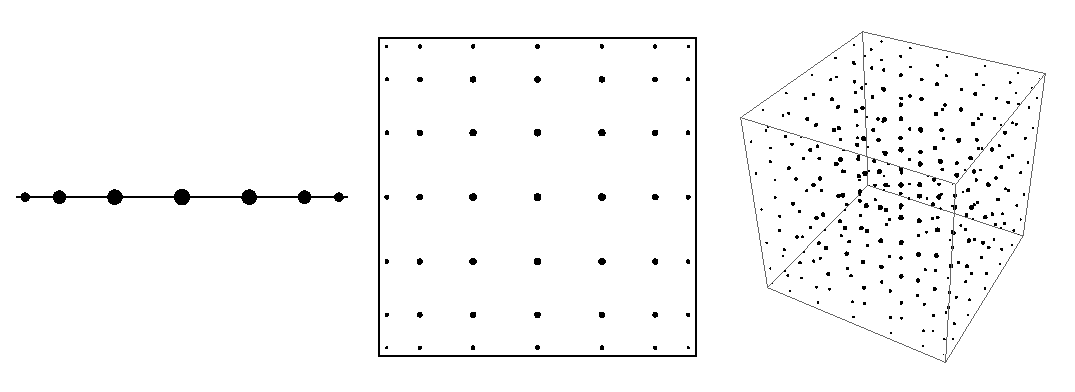
\includegraphics[height=0.25\textheight]{tensorproduct_quadrature.eps}
		\caption{StÜtzstellen eines 1D 7--Punkt--Gauss--Legendre--Verfahrens und entsprechender Tensor--Produkt--Verfahren fÜr 2 bzw. 3 Dimensionen. Die Gewichte der StÜtzstellen sind durch ihre Grö"se kenntlich gemacht.}
		\label{fig:tensorproduct}
	\end{figure}
	
	\subsection{einfache Monte--Carlo--Integration}
	Bei der Monte--Carlo--Integration ziehen wir $N$ zufÄllige, gemÄ"s einer Wahrscheinlichkeitsdichte $p$ verteilte StÜtzstellen $[X_i|i\in\{1,\dots,N\}]$ in $\Omega$ und schÄtzen dann den Wert des Integrals (\ref{eq:integration_problem}) mit
	\begin{equation}
		{\tilde I}_d^{\,\text{MC}}=\frac{1}{N}\sum_{i=0}^{N-1} \frac{f(X_i)}{p(X_i)}
		\label{eq:mc_integral}
	\end{equation}
	ab. Im Falle unseres $d$--dimensionalen EinheitswÜrfels $\Omega=[0,1]^d$ können wir besipielsweise jede StÜtzstelle aus $d$ gleichförmig auf dem Einheitsintervall $[0,1]$ verteilten Zufallszahlen $U_i$ durch einfache Tupelbildung
	$$X_i:=(U_{d i},\dots,U_{d(i+1)-1})$$
	gewinnen. Aber auch fÜr allgemeine Integrationsgebiete $\Omega$ kann das Verfahren genauso angewandt werden, solange ein passendes Integrationsma"s $\mu$ und ein Wahrscheinlichkeitsma"s $P$ existieren, so dass $$P(D)=\text{Pr}(x\in D)$$ fÜr jede me"sbare Menge $D\subset\Omega$ gilt. Die entsprechende Wahrscheinlichkeitsdichte $p$ lÄsst sich mit Hilfe der {\em Radon--Nikodym--Ableitung} $$p(x)=\frac{dP}{d\mu}(x)$$
	einfÜhren, wobei $p$ dann einfach eine Funktion ist, fÜr die $$P(D)=\int_D p(x)d\mu(x)$$ gilt.
	Von der Erwartungstreue des SchÄtzers (\ref{eq:mc_integral}) fÜr unser Integral (\ref{eq:integration_problem}) können wir uns mit \citep[][2.4]{Veach:1997p9136}
	\begin{align*}
		E[{\tilde I}_d^{\,\text{MC}}] &=E\left[\frac{1}{N}\sum_{i=0}^{N-1}\frac{f(X_i)}{p(X_i)}\right] \\
			&= \frac{1}{N}\sum_{i=0}^{N-1}E\left[\frac{f(X_i)}{p(X_i)}\right] \\
			&= \frac{1}{N}\sum_{i=0}^{N-1}\int_\Omega \frac{f(X_i)}{p(X_i)}p(X_i)\,d\mu(x) \\
			&= \int_\Omega f(x)\,d\mu(x)\\
			&= I
	\end{align*}
	leicht Überzeugen.
	
	\subsection{Konvergenzraten}\label{subsec:integrationsproblem_comparison}
	Wir wollen nun die Konvergenzraten der Tensor--Produkt--Verfahren mit der Konvergenzrate des einfachen Monte--Carlo--SchÄtzers (\ref{eq:mc_integral}) vergleichen. Zur Konstruktion eines Vertreters der Tensor--Produkt--Verfahren verwenden wir beispielhaft das Newton--Cotes--Verfahren. In \citep[][3.1.4]{Stoer:2005p10586} wird als Ab\-schÄt\-zung fÜr den Fehler eines Verfahrens $p$--ter Ordnung (d.h. ein Verfahren, das alle Polynome bis zum Grad $p$ exakt integriert) und Schrittweite $h(\approx\frac{b-a}{N}=\mathcal{O}(N^{-1}))$ der StÜtzstellen
	\begin{equation}
		\int_a^b P_n(x)-f(x)dx=h^{p+1}K f^{(p)}(\xi),\quad\xi\in(a,b)
		\label{eq:quadrature_error}
	\end{equation}
	angegeben, wobei $n$ die Anzahl der StÜtzstellen, $P_n$ das Interpolationspolynom fÜr die StÜtzstellen und K eine Konstante ist. Gauss--Legendre--Verfahren sind von der Ordnung $2n-1$, d.h. die Konvergenzrate dieser $n$--Punkt--Formel ist demnach von der Grö"senordnung $\mathcal{O}(h^{2n})=\mathcal{O}(N^{-2n})$.\footnote{$N$ bezeichnet die Anzahl der StÜtzstellen fÜr das gesamte Integrationsintervall. Der SchÄtzwert fÜr das Integral wird dann durch $\frac{N}{n}$--maliges Anwenden der $n$--Punkt--Formel berechnet}
	Durch Bildung der entsprechenden $d$--dimensionalen Tensor--Produkt--Regel Ändert sich die Konvergenzrate in Bezug auf die Schrittweite $h$ nicht. Da unsere $N$ StÜtzstellen sich nun aber auf ein $d$--dimensionales Gitter verteilen, teilt sich das Volumen unseres $d$--dimensionalen EinheitswÜrfels in $N$ WÜrfel mit einem Volumen von jeweils $h^d$ auf, d.h. fÜr die Schrittweite folgt
	$$\mathcal{O}(1)=V=N h^d \Rightarrow h=\mathcal{O}\left(\left(\frac{1}{N}\right)^{1/d}\right)=\mathcal{O}\left(N^{-1/d}\right)$$	
	und damit fÜr die Konvergenzrate in Bezug auf die GesamtstÜtzstellenzahl
	$$\mathcal{O}(h^{2n})=\mathcal{O}(N^{-2n/d}).$$
	Dies bedeutet, dass Tensor--Produktverfahren mit steigender Dimension des Integrationsgebietes an Effizienz verlieren. Bei hochdimensionalen Problemen kann dies kaum durch Verfahren höherer Ordnung ausgeglichen werden, da Verfahren höherer Ordnung, wie oben in (\ref{eq:quadrature_error}) zu sehen, auch grö"sere Anforderungen an die Glattheit der Funktion stellen. Au"serdem kann die exponentiell steigende Anzahl $N \geq n^d$ mindestens nötiger Funktionsaufrufe zu einem Problem werden. Der Effekt wird bei steigender Dimension und Ordnung des Verfahrens nur noch schlimmer, was ein Ausgleichen der schlechteren Konvergenzrate bei höheren Dimensionen durch Erhöhen der Ordnung des Verfahrens schnell praktisch unmöglich werden lÄsst. Dies wird hÄufig als {\em Curse~of~Dimensionality} (Fluch der DimensionalitÄt) bezeichnet.
	
	Bei der Monte--Carlo--Integration können wir die Konvergenzrate anhand der Varianz unseres Monte--Carlo--SchÄtzers (\ref{eq:mc_integral}) bestimmen \citep[][2.4.1]{Veach:1997p9136}. Nennen wir der Übersicht wegen
	$$Y_i=\frac{f(X_i)}{p(X_i)}$$
	und den MC--SchÄtzer mit $N$ gezogenenen Werten
	$$F_N=\frac{1}{N}\sum_{i=0}^{N-1} Y_i.$$
	Dann gilt fÜr die Varianz eines beliebigen Samples
	\begin{equation}
		V[Y_i]=E[(Y_i-E[Y_i])^2]=E[Y_i^2]-E[Y_i]^2=\int_\Omega \frac{f(x)^2}{p(x)}d\mu(x)-I^2.
		\label{eq:mc_variance}
	\end{equation}
	Da die Werte unabhÄngig gezogen sind, gilt fÜr die Varianz des SchÄtzer mit $N$ Werten
	$$V[F_N]=V\left[\frac{1}{N}\sum_{i=0}^{N-1}Y_i\right]=\frac{1}{N^2}V\left[\sum_{i=0}^{N-1}Y_i\right]=\frac{1}{N^2}\sum_{i=0}^{N-1}V[Y_i]=\frac{1}{N}V[Y_i],$$
	d.h. die Varianz des SchÄtzers sinkt invers mit der Anzahl $N$ an gezogenen Werten. Daraus folgt sofort die Standardabweichung
	\begin{equation}
		\sigma[F_N]=\frac{1}{\sqrt{N}}\sigma[Y_i],
		\label{eq:mc_standarddeviation}
	\end{equation}
	was einer Konvergenzrate von $\mathcal{O}(N^{-1/2})$ entspricht. Die Konvergenzrate des Monte--Carlo--SchÄtzers ist im Gegensatz zur Konvergenzrate der Tensor--Produkt--Verfahren also unabhÄngig von der Dimension des Integrationsgebietes, d.h. das Verfahren leidet {\em nicht} unter dem {\em Curse~of~Dimensionality}! Au"serdem mussten wir nirgendwo Bedingungen an die Glattheit der Funktion stellen, was bei Funktionen mit DiskontinuitÄten von Vorteil ist.
	
	Zusammenfassend können wir also feststellen, dass Monte--Carlo--Integration bei hochdimensionalen Integrationsproblemen und Funktionen mit DiskontinuitÄten klar gegenÜber klassischen Tensor--Produktverfahren vorzuziehen ist. FÜr niedrigdimensionale ($d\lessapprox 7$) Gebiete mit glatten Integranden sind die klassischen Methoden hingegen besser geeignet.
	
	
	\section{Importance--Sampling}\label{subsec:importancesampling}
	Wir sind bei unserem MC--SchÄtzer (\ref{eq:mc_integral}) nicht darauf beschrÄnkt eine gleich\-för\-mi\-ge Wahrscheinlichkeitsdichte $p$ zu wÄhlen. Es kann die Effizienz des Verfahrens sogar betrÄchtlich verbessern, wenn wir eine geeignete Wahrscheinlichkeitsdichte $p$ wÄhlen. Schauen wir uns daher die Formel (\ref{eq:mc_variance}) fÜr die Varianz, die es zu minimieren gilt, nochmal an, um zu verstehen, was ``geeignet'' bedeutet. Nimmt die Wahrscheinlichkeitsdichte beispielsweise die ideale Form
	\begin{equation}
		p(x)=\frac{|f(x)|}{\int_\Omega |f(z)|d\mu(z)}
		\label{eq:ideal_importance_pdf}
	\end{equation}
	an, kann man mit der {\em Jensenschen~Ungleichung} zeigen, dass dann das Integral in (\ref{eq:mc_variance}) und damit die Varianz insgesamt minimal wird. Nimmt $f$ keine negativen Werte an, verschwindet die Varianz dieses SchÄtzers sogar, da in (\ref{eq:mc_integral}) dann nur noch Über die konstante Lösung (in Form der Normierungskonstanten) gemittelt wird. Wenn wir das Normierungs--Integral im Nenner von (\ref{eq:ideal_importance_pdf}) lösen könnten, wÄre allerdings auch die ursprÜngliche Integration (\ref{eq:integration_problem}) kein Problem! Daher suchen wir in der Praxis nach einem $p$, das möglichst Ähnlich zu $|f|$ und gleichzeitig normierbar ist.
	

		\section{Monte--Carlo--Markov--Chain--Verfahren}
	Bisher sind wir bei unserem Monte--Carlo--Sch"atzer (\ref{eq:mc_integral}) von einer zugrundeliegenden Stichprobe aus $N$ unabh"angigen und identisch gem"a"s $p$ verteilten St"utzstellen ausgegangen, deren zugeh"rige Funktionswerte gemittelt als Sch"atzer f"ur den Wert des Integrals (\ref{eq:integration_problem}) dienen. Wenn wir aber unsere Funktionswerte in jedem Fall mitteln, dann ist die Unabh"angigkeit der gezogenen St"utzstellen nicht relevant, da die Reihenfolge, in der sie gezogen werden, den Mittelwert nicht beeinflusst. Essentiell ist also lediglich, dass sie identisch gem"a"s $p$ verteilt sind.
	
	Diese Freiheit nutzen sogenannte Monte--Carlo--Markov--Chain--Verfahren (MCMC--Verfahren). Sie stellen ein Verfahren dar, um aus einem Zustandsraum $\Omega$ gem"a"s einer gegebenen Wahrscheinlichkeitsdichte $p$ verteilte Werte zu ziehen. Dies wird durch die Konstruktion eines Zufallspfads ({\em random~walk}) im Zustandsraum, dirigiert durch eine Markov--Kette, erreicht. Dabei mu"s sichergestellt werden, da"s die so erzeugten Werte auch gem"a"s $p$ verteilt sind und insbesondere jeder Punkt im Zustandsraum, auf dem $p$ nicht verschwindet, auch erreicht werden kann.
	
	Wie im n"achsten Abschnitt gezeigt wird, ist dies mit erstaunlich wenig Aufwand m"oglich. Die Kombination aus Vielseitigkeit, M"achtigkeit und Einfachheit hat MCMC--Verfahren in vielen Bereichen\footnote{Beispiele finden sich u.a. in der statistischen Physik, in der Finanzmathematik und zur Berechnung von A--posteriori--Wahrscheinlichkeiten in der Bayes'schen Statistik \citep{Geweke:1989p10465}, z.B. mit Anwendungen in der Bioinformatik und Medizin. Weitere interessante und ungew"ohnliche Anwendungen finden sich in \citep{Diaconis:2009p4122}} zu einem Hauptverfahrensbestandteil gemacht.
	
	
	\subsection{Metropolis--Hastings--Algorithmus}
	Unter den MCMC--Verfahren ist eines der bekanntesten der {\em Metropolis--Hastings--Algorithmus} (MH), der durch eine Arbeit in der statistischen Physik von \citet{Metropolis:1953p3364} in einer einfachen Form vorgestellt und sp"ater durch \citet{Hastings:1970p3387} verallgemeinert wurde.

	Beim MH--Algorithmus ziehen wir aus einem Zustandsraum $\Omega$ Elemente $x \in \Omega$ gem"a"s der (nicht notwendigerweise normierten!) Wahrscheinlichkeitsdichte $f : \Omega \rightarrow \mathbb{R}_{\geq 0}$. Die Elemente werden dabei mit einem Zufallspfad durch den Zustandsraum generiert. Wir ver"andern dazu den aktuellen Zustand $x$ nach einem frei w"ahlbaren Schema (im Folgenden Mutation genannt) in einen neuen Zustand $x'$.
	Dabei stellen wir folgende Bedingungen an eine Mutation:
	\begin{itemize}
		\item{wenn der "Ubergang von Zustand $x$ nach $x'$ m"oglich ist, muss auch der "Ubergang zur"uck von $x'$ nach $x$ m"oglich sein}
		\item{es muss jeder Zustand $x \in \Omega$ durch eine Kette von "Uberg"angen erreichbar sein (Ergodizit"at)}
		\item{Die "Ubergangswahrscheinlichkeit $T(x'|x)$ durch unser Mutations--Schema von Zustand $x$ zum Zustand $x'$ zu kommen muss f"ur gegebenes $x$ und $x'$ berechenbar sein}
	\end{itemize}
	Mutationen sind also, etwas formaler formuliert, bedingte Wahrscheinlichkeitsverteilungen, die durch das Herkunftselement parametrisiert sind, nicht normiert sein m"ussen und f"ur die
	$$\forall x,x'\in\Omega : \quad T(x'|x)>0 \Leftrightarrow T(x|x')>0$$
	wahr ist. Hierin k"onnen wir eine Parallele zum {\em Importance Sampling} aus Abschnitt \ref{subsec:importancesampling} entdecken, bei dem wir auch die A--priori--Wahr\-schein\-lich\-keits\-ver\-tei\-lung, aus der die Werte gezogen werden, selber w"ahlen k"onnen ohne das Ergebnis der Integration zu verf"alschen. W"ahrend wir uns beim Importance Sampling allerdings f"ur eine einzige Verteilung zur Generierung der gesamten Stichprobe entscheiden m"ussen, haben wir beim {\em MH--Algorithmus} die M"oglichkeit, f"ur jeden aktuellen Zustand eine eigene Verteilung festzulegen aus der ein Vorschlag f"ur den neuen Zustand gezogen wird.
	Das bedeutet, Mutationen k"onnen (und sollten) f"ur effizientes und verl"assliches Verhalten an das spezifische Samplingproblem angepasst werden indem die Eigenschaften der interessierenden Wahrscheinlichkeitsdichte $f$ und des Zustandsraumes $\Omega$ miteinbezogen werden. Sind beispielsweise exakte oder n"aherungsweise g"ultige Invarianten von $f$ bez"uglich seiner Zustandsraumkoordinaten bekannt, k"onnen diese genutzt werden, um Samples "ahnlicher Wahrscheinlichkeitsdichte aber gering korrelierten Zustandsraumkoordinaten zu ziehen.
	
		
	\paragraph{Detailed Balance:}
	Da die Mutation, mit der wir den neuen Zustand generieren, nichts mit der Wahrscheinlichkeitsdichte $f$ zu tun haben mu"s, brauchen wir eine M"oglichkeit die Verteilung der Zust"ande gem"a"s $f$ trotzdem sicherzustellen.
	
	Betrachten wir eine gro"se Zahl von gleichartigen aber unabh"angigen Markov--Ketten, die alle mit einer gewissen Wahrscheinlichkeit $p(x'|x)$ vom Zustand $x$ in den Zustand $x'$ "ubergehen, dann ist eine M"oglichkeit eine station"are Zustandsdichte $f$, gemittelt "uber die aktuellen Zust"ande aller Markov--Ketten, zu erreichen, zu verlangen, da"s
	\begin{equation}
		\forall x,x' \in \Omega :\quad f(x)p(x'|x) = f(x')p(x|x')
		\label{eq:dynamic_equlibrium}
	\end{equation}
	({\em =Detailed Balance}) gilt, d.h. da"s die "Ubergangsraten zwischen zwei beliebigen Zust"anden sich im dynamischen Gleichgewicht befinden.
	Da $T$ die "Ubergangswahrscheinlichkeiten aber schon festlegt, behalten wir uns das Recht vor, einen durch Ziehen aus $T$ vorgeschlagenen Zustands"ubergang nur mit der Wahrscheinlichkeit $a(x'|x)$ anzunehmen und ansonsten abzulehnen,	um {\em Detailed Balance} sicherstellen zu k"onnen:
	\begin{equation}
		p(x'|x) = T(x'|x)a(x'|x)
		\label{eq:acceptance_prob_intro}
	\end{equation}
	\begin{equation}
		(\ref{eq:dynamic_equlibrium}) \stackrel{(\ref{eq:acceptance_prob_intro})}{\Longrightarrow}
		\forall x,x' \in \Omega :\quad f(x)T(x'|x)a(x'|x) = f(x')T(x|x')a(x|x')
		\label{eq:detailedbalance}
	\end{equation}
	Dies l"asst noch immer verschiedene M"oglichkeiten zu, die Akzeptanzwahrscheinlichkeit zu bestimmen. Eine effiziente und dadurch beliebte Wahl ist dabei Folgende: ist $f(x')>f(x)$ nehmen wir den neuen Zustand auf jeden Fall an, ansonsten mit der Wahrscheinlichkeit $(f(x')T(x|x'))/(f(x)T(x'|x))$. Dies l"asst sich zusammenfassen zu
	\begin{equation}
		a(x'|x)=\text{min}\left(1,\frac{f(x')T(x|x')}{f(x)T(x'|x)}\right)
		\label{eq:acceptanceratio}
	\end{equation}
	Diese Wahl der Akzeptanzwahrscheinlichkeit erf"ullt die Detailed--Balance--Bedingung (\ref{eq:detailedbalance}).
	
	
	
	\paragraph{Pseudocode:}
	In Pseudocode sieht der Algorithmus dann wie folgt aus:
	\begin{algorithmic}
		\STATE $x_1 \leftarrow$ Anfangszustand
		\FOR{$i=1$ to $N$}
			\STATE $x'\leftarrow$ ziehe Wert gem"a"s $T(x'|x_i)$
			\STATE $a(x'|x_i) \leftarrow \text{min}\left(1, \frac{f(x')T(x|x')}{f(x)T(x'|x)}\right)$
			\STATE $u\leftarrow$ Zufallszahl aus $[0,1]$
			\IF{$u < a(x'|x_i)$}	\STATE $x_{i+1} \leftarrow x'$
			\ELSE	\STATE $x_{i+1} \leftarrow x_i$
			\ENDIF
	  \ENDFOR
	\end{algorithmic}
	Als Ergebnis erhalten wir eine Liste von Werten, die gem"a"s $f$ verteilt sind.
	Die Tatsache, da"s die Normierung von $f$ f"ur die Funktion des Verfahrens nicht notwendig ist, kann einerseits von Vorteil sein, und bei bestimmten Problemen die effiziente Generierung einer Stichprobe erst m"oglich machen, sie bedeutet allerdings, da"s wir uns bei Bedarf eine Normierung auf andere Weise beschaffen m"ussen, da die gezogenen Werte ebenfalls nicht normiert sind. Die Werte sind ausserdem nicht unabh"angig, sondern im Gegenteil h"aufig stark korreliert.

	\paragraph{Konvergenz:}Bei klassischer Monte--Carlo--Integration hatten wir in Abschnitt \ref{subsec:integrationsproblem_comparison} gezeigt, da"s bei einer Standard--Abweichung eines Wertes von $$\sigma^*:=\sigma\left[\frac{f(X_i)}{p(X_i)}\right]$$ die Standard--Abweichung des Mittelwertes von N unabh"angig gezogenen Werten $\sigma^*/\sqrt{N}$ betr"agt. Sind die Werte hingegen korreliert, gilt f"ur die Standard--Abweichung des Mittelwertes die Absch"atzung \citep[siehe][VII.\;\S3(8)]{Renyi:1964p10655}
	$$\sigma\leq \sigma^*\sqrt{\frac{1+2\sum_{i=1}^N R(i)}{N}},$$
	wobei $R(|j-i|)\leq 1$ eine obere Schranke f"ur die Korrelation zwischen $f(X_i)/p(X_i)$ und $f(X_j)/p(X_j)$ ist.
	Eine gro"se Korrelation kann sich also negativ auf die Konvergenzrate des Mittelwertes (und anderer statistischer Kenngr"o"sen) auswirken. Daher gilt es bei der Konstruktion einer Mutation zwei Aspekte gegeneinander abzuw"agen: einerseits ist es w"unschenswert in einem Mutationsschritt m"oglichst ``gro"se Schritte'' zu machen um die Korrelation der Werte kleinzuhalten, andererseits ist es in selten gezogenen Bereichen mit hohem Beitrag w"unschenswert kleine Schritte zu machen, um diesen Bereich gut abzudecken. W"ahrend ersteres Verfahren meist mit einer kleinen Akzeptanzwahrscheinlichkeit einhergeht, f"uhren kleine Mutationen tendenziell zu hohen Akzeptanzwahrscheinlichkeiten. Beide ziehen aber in zu extremer Form hohe Korrelation der Samples nach sich, bei zu gro"sen Schritten aufgrund der geringen Akzeptanzwahrscheinlichkeit und daher mehrfacher Gewichtung desselben Samples, bei zu kleinen Schritten aufgrund der gro"sen "Ahnlichkeit der vorgeschlagenen Samples. Daher sind sowohl zu hohe als auch zu kleine Akzeptanzwahrscheinlichkeiten meistens ein Zeichen suboptimalen Samplings. In \citep{Roberts:1997p5198} wird zur Steuerung der Mutationsst"arke f"ur die Akzeptanzwahrscheinlichkeit ein anzustrebender Wert von $\approx 0.23$ bei hochdimensionalen Problemen empfohlen.

	
	
	\subsection{Generalisierter Metropolis--Hastings--Algorithmus}
	Wir haben in Abschnitt \ref{subsec:importancesampling} festgestellt, da"s die Effizienz des einfachen Monte--Carlo--Sch"atzers erheblich verbessert werden kann, wenn f"ur {\em Importance Sampling} eine geeignete A--priori--Wahrscheinlichkeitsdichte $p$ bekannt und samplebar ist. Parallel dazu haben wir im vorigen Abschnitt gesehen, da"s es auch f"ur ein effizientes Funktionieren des {\em Metropolis--Hastings--Algorithmus} wichtig ist, die Mutationen an das Problem anzupassen.


		\chapter{Monte--Carlo--Strahlungstransport}\label{sec:mc_radiativetransfer}
	\section{Pfadgenerierung}
	\subsection{Raycasting}
	\subsection{Distanzsampler}
	TODO: uniform depth sampler, uniform attenuation sampler, enforced uniform attenuation sampler
	
	TODO: Pfadgenerierung, Sch"atzer
	
	
	\chapter{Testf"alle und Resultate}
	\section{Homogene streuende Kugel}
	TODO: Motivation? tau=0.01,1,10
	\subsection{analytische L"osung}
	\subsection{Resultate}
	TODO: Vergleich mit analytischer L"osung und MC3D (Ergebnis+Geschwindigkeit)
	\section{Einfaches Scheibenmodell}
	\subsection{Resultate}
	TODO: Vergleich mit MC3D (Ergebnis und Geschwindigkeit)
	\section{Einordnung der Resultate}
	TODO: Gesamtvergleich zwischen MC3D und PIRaTE
	
	\chapter{Programmbeschreibung}
	TODO: Programmbeschreibung in Worten bzw. Pseudocode, Modulbeschreibung, Details in evtl. Anhang auslagern.
	
	\chapter{Zusammenfassung und Ausblick}
	TODO: Ausblick: Normierung, physikalisch relevante Streuphasenfunktionen, polychromatische Bilder/SEDs

\backmatter
	\bibliographystyle{chicago}
	\bibliography{bibliography}

\end{document}